\documentclass{article}

\usepackage[margin=1in]{geometry}
\usepackage{amsmath}
\usepackage{amssymb}
\usepackage{amsthm}
\usepackage{graphicx}
\theoremstyle{definition}
\newtheorem{definition}{Definition}[section]
 
\title{Braid Cryptosystem Notes}
\date{\today}



\begin{document}
	\maketitle
	
	\section{Braid Cryptographic System}
	
	\subsection{Braids}
	%TODO: who created braids and operations on braids
	In this section we will explain the mathematics behind a braid group. A braid group has braids as the set and concatenation as the group operation written as $<B_n,||>$ where $n$ is the number of strands and 

\begin{definition} 
$B_n=\{\sigma_1,...,\sigma_{n-1}:\sigma_i\sigma_j\sigma_i=\sigma_j\sigma_i\sigma_j\ \textrm{if}\ |i-j|=1\ \textrm{and}\ \sigma_i\sigma_j=\sigma_j\sigma_i\ \textrm{if}\ |i-j|>1\}$
\end{definition}
 
A braid group is infinite and nonabelian meaning that the elements do not commute such that:
$a,b \in B_n: \ ab\neq ba$. Note that for $n$ strands there are $n-1$ generators represented by $\sigma$. A braid is the concatenation of generators. A positive generator, $\sigma_i^+$, corresponds to crossing left over right and a negative generator corresponds to crossing right over left, $\sigma_i^-$. 

\begin{figure}[hbp!]
\centering
  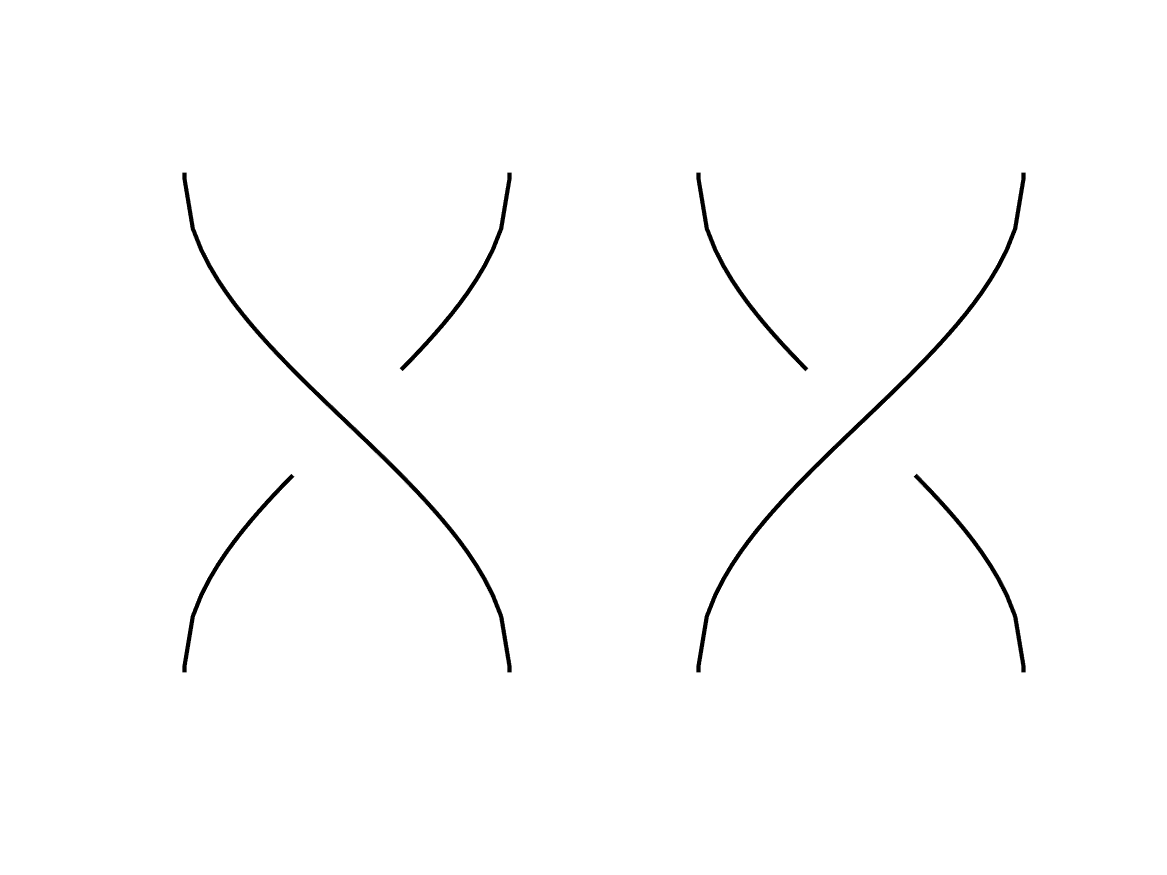
\includegraphics[width=0.2\linewidth]{./Pictures/gen_pos_neg.png}
  \caption{$\sigma_i^+$,$\sigma_i^-$}\label{fig:graph}
\end{figure}


For example the braid $b \in B_3: \ b=\sigma_2^+ \sigma_1^+ \sigma_2^- \sigma_1^-$ is the following:
	
	\begin{figure}[hbp!]
\centering
  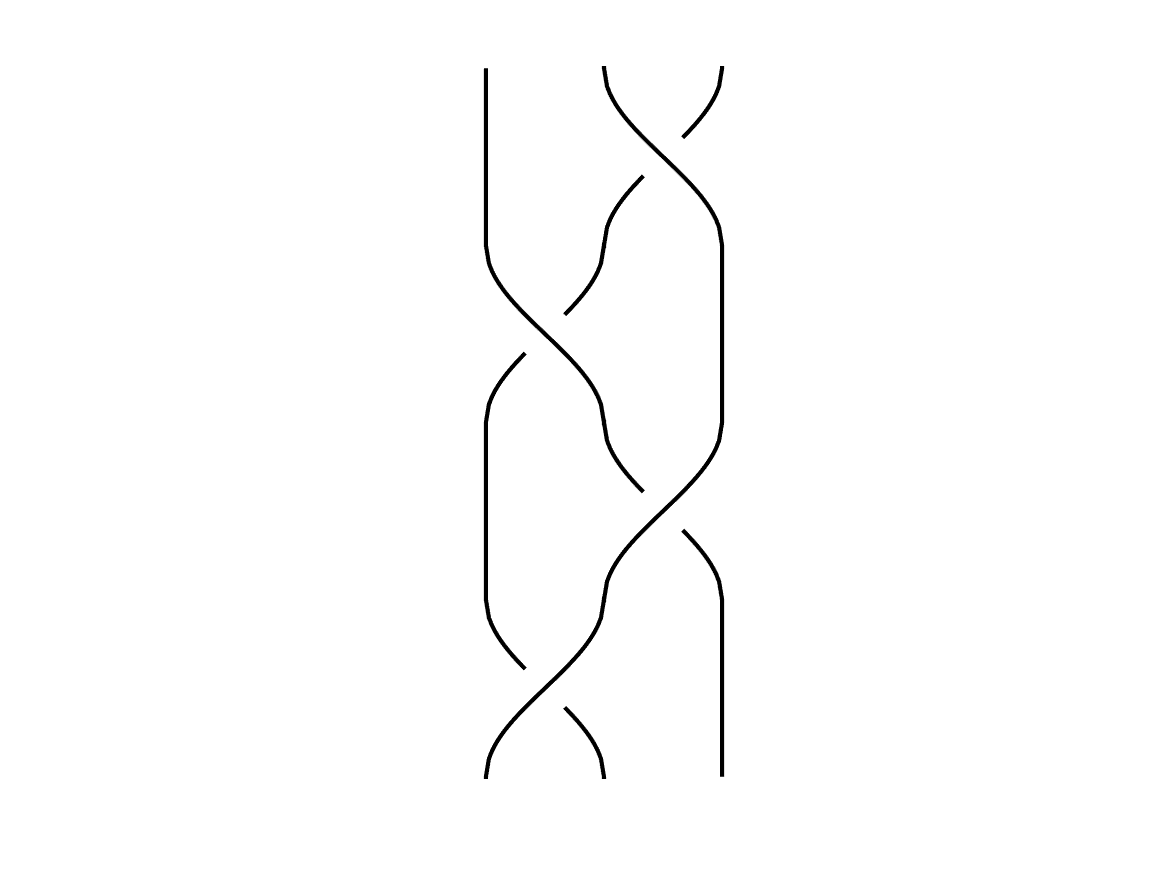
\includegraphics[width=0.2\linewidth]{./Pictures/example_braid.png}
\end{figure}
	
	
	
	
	
	
	\subsubsection{Left and Right Canonical Forms}
	
	For any $w \in B_n$ $\exists$ a unique representation called the left canonical form.
	
	\begin{align*}
		&w = \Delta^u A_1 A_2 ... A_l, u \in Z', A \in \Sigma_n \text{ without the following elements } \{ e, \Delta \} \\
		&\text{where } A_i A_{i+1} \text{is left weighted for } 1 \leq i \leq l - 1 \\
		&\text{where } \Sigma_n \text{ is the set of all permutation braids.}
	\end{align*}
	
	\subsection{Sub-Groups of the Braid Group}
	There are two commuting subgroups of $B_n$.
	
	\begin{align*}
		LB_n < B_n & \text{ generated by } \{ \sigma_1 , ..., \sigma_{ \left[ n/2 \right] } \}  \\
		UB_n < B_n & \text{ generated by } \{ \sigma_{ n/2 + 1 }, ..., \sigma_{n-1} \} \\
		a \in B_n & \text{ commutes w/} b \in UB_n : ab = ba 
	\end{align*}
	
	Notice how $\sigma_3$ is missing, we do this in order to be able to commute the upper and lower group.
	
	We do this using the second part of the braid definition
	%TODO: latex braid definition and reference 2nd part
	
	\subsection{Braid Cryptographic System}
	Let's define the Braid Cryptographic System.
	\begin{align*}
	n &: \text{the Braid index} \\
	l &: \text{the Canonical Index}
	\end{align*}
	
	\subsubsection{Commuter-based Key Agreement}
	%TODO: explain conjugacy problem parallel to factoring problem
	There are many variants of the conjugacy search problem.
	
	\subsubsection{Generalized Conjugacy Search}
	Given: $x,y \in B_n \text{ s.t. } y=a^{-1}xa \text{ for some } a \in LB_n$ \\
	Find: $b \in LB_n \text{ s.t. } y = b^{-1}xb$ \\
	(note: can replace $LB_n$ w/ $UB_n$)
	
	\section*{Deliverables}
	\subsection*{11/21/2019}
	\begin{enumerate}
		\item Finish Notes (TP) (COMPLETE)
		\item  Install/Demo CBraid (reference 6 of Anandam) (JL, BK, TP) (COMPLETE)
		\item Learn Cryptosystem part (RM) (COMPLETE)
	\end{enumerate}


	
\end{document}